\chapter{Sampling and SFZ}
\label{chap:sampling-sfz}

A synth computes sound; a sampled instrument plays recordings. Yeban's sampling side is built around SFZ: a text file describing which key range, which velocity range, which audio file, and how to transpose it. The audio stays on disk. Understanding that split is how you tell "no sound" apart from a missing file, an uncovered key, or the wrong entry point.

\section{What SFZ is, and what it is not}

SFZ is a text definition file. It does not contain PCM, and it does not pack a whole sample library into the project; it lists regions and sample paths. Yeban parses the SFZ, flattens the region table into a playable instrument, and chooses regions by note and velocity. The project stores only the path of the SFZ bound to a track, so the project file stays small, but moving machines, deleting a library, or relocating samples can break that path.

Only one main source sounds on a track: the dispatch order is \textbf{drum machine > SFZ > poly synth}. If a track carries a drum machine, an SFZ, and a synth at once, the drum machine wins and the other two are ignored. That is the established "one main source per track" rule, not a bug.

\section{Three entry points, three destinations}

Several places in the UI say "SFZ" or "sample library"; they do not do the same thing:

\begin{table}[htbp]
\centering
\small
\begin{tabular}{@{}p{0.28\linewidth}p{0.34\linewidth}p{0.30\linewidth}@{}}
\hline
Entry point & Actual action & Binds current track? \\
\hline
Device rack "+ Load SFZ" / left-library sample entry & Opens the instrument manager; choosing an item loads it onto the current track & Yes, writes the track sampler \\
Top module bar "Load SFZ" & Chooses an SFZ as the export/audition source and reports regions plus a probe reading & No, does not change track binding \\
File menu "Load SFZ sound library..." & Same module action as the top bar & No, current implementation does not write track binding \\
\hline
\end{tabular}
\caption{What the three SFZ entry points actually do}
\label{tab:sfz-entry}
\end{table}

To put an instrument on a track, use the device-rack empty-state button or the left-library sample entry: select an item and load it onto the current track; the project commits a \texttt{SetTrackSampler}. The top "Load SFZ" is the bypass for "use this source for the whole project's audition/export": it keeps the instrument in a memory slot for the next export and does not replace the current track's source. If its default path has no file, it opens the instrument manager instead of reporting a jargon error.

\section{Key ranges, root keys, and velocity layers}

Every SFZ region answers at least four questions: which keys it covers (\texttt{lokey}/\texttt{hikey}), which velocities it covers (\texttt{lovel}/\texttt{hivel}), where its root is (\texttt{pitch\_keycenter}, default 60), and which file it plays (\texttt{sample}). A note triggers only inside the region; when several regions cover the same key and velocity, they layer. That is what layered sampling means.

\begin{center}
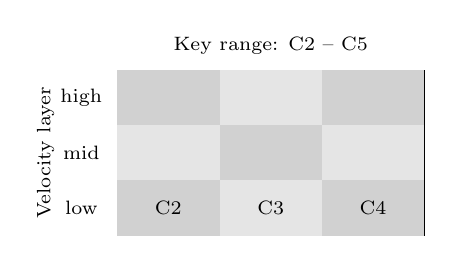
\begin{tikzpicture}[font=\scriptsize, x=13mm, y=7mm]
  \foreach \x in {0,1,2,3} { \draw (\x,0) -- (\x,3); }
  \foreach \y in {0,1,2,3} { \draw (0,\y) -- (3,\y); }
  \node at (1.5,3.45) {Key range: C2 -- C5};
  \node[rotate=90] at (-0.7,1.5) {Velocity layer};
  \node at (-0.35,2.5) {high};
  \node at (-0.35,1.5) {mid};
  \node at (-0.35,0.5) {low};
  \fill[black!18] (0,0) rectangle (1,1);
  \fill[black!10] (1,0) rectangle (2,1);
  \fill[black!18] (2,0) rectangle (3,1);
  \fill[black!10] (0,1) rectangle (1,2);
  \fill[black!18] (1,1) rectangle (2,2);
  \fill[black!10] (2,1) rectangle (3,2);
  \fill[black!18] (0,2) rectangle (1,3);
  \fill[black!10] (1,2) rectangle (2,3);
  \fill[black!18] (2,2) rectangle (3,3);
  \node at (0.5,0.5) {C2};
  \node at (1.5,0.5) {C3};
  \node at (2.5,0.5) {C4};
\end{tikzpicture}
\end{center}

Each cell is one "key range × velocity layer" group. A real SFZ need not fill the whole table: if only C3 at medium velocity is written, C4 has no sound; if only high velocity is written, a light touch does not trigger. When "some keys sound, others do not", check region coverage before suspecting the engine.

The root key determines transposition. If a sample was recorded at C3 but \texttt{pitch\_keycenter} says 60 (C4), playing C3 sounds a whole octave low. Yeban's load report performs notation adaptation: when the file writes key names and the sample has no embedded root, evidence is insufficient and no automatic shift happens; the receipt warns that the octave may be off. The project model supports \texttt{note\_octave\_override}, but the current UI has no separate octave knob, so do not expect one click to fix every library.

Velocity response comes from \texttt{amp\_veltrack} (default 100\%, range $-100$–$100$) plus an optional \texttt{amp\_velcurve\_N} point table; key-dependent loudness comes from \texttt{amp\_keytrack} (default 0 dB/key, range $-96$–$12$). Most libraries need neither changed; if an entire velocity layer is too loud or soft, inspect the library first, then consider changing the Yeban side.

\section{Supported files and fallbacks}

Yeban dispatches samples by suffix: \texttt{.wav}/\texttt{.wave} go through PCM/float WAV decoding; other common formats (FLAC, OGG, and so on) go through the general decoder. Both legs preserve channels, and samples with more than two channels are explicitly rejected rather than silently folded to mono.

\begin{table}[htbp]
\centering
\small
\begin{tabular}{@{}p{0.30\linewidth}p{0.60\linewidth}@{}}
\hline
Situation & Yeban's behavior \\
\hline
Mono/stereo WAV, FLAC, OGG, etc. & Decodes normally; stereo keeps left and right \\
Sample rate differs from project & No resampling; playback-rate conversion, original rate kept in the report \\
Sample missing or unreadable & Falls back to a 440 Hz in-memory sine and lists the path under missing; not a silent success \\
More than two channels & Explicitly rejects that sample \\
\texttt{sample=*silence} & Built-in silent pseudo-sample: the region exists and triggers, but produces no sound \\
\texttt{\#include} missing or unmatched & Loading continues; each issue goes into include\_issues \\
\hline
\end{tabular}
\caption{How sample reads succeed and fail}
\label{tab:sfz-samples}
\end{table}

The fallback sine is a diagnostic signal, not a substitute timbre. A clean 440 Hz sine means the sample was not read; inspect the missing list and fix the path or file instead of reaching for EQ.

Each track's SFZ voice pool holds 16 voices. Beyond that, the existing steal policy replaces older voices and accumulates a steal count. That ceiling is enough for ordinary arrangements, but large ensembles or long release overlaps should expect stealing rather than infinite polyphony.

\screenshot{sample-library-picker}{The instrument manager is open, installed instruments are listed, an entry has a load-to-current-track action, and the current track is MIDI.}

\section{Sample-library management}

Yeban manages a single sample-library root outside the project directory. When no library is installed, the device-rack sample-library button reads "Download sample library (about 9.4 GiB)"; once installed, the same button becomes "Verify sample library". Downloads happen only when the user clicks, never silently in the background.

A pack is verified by SHA-256 and size before installation; a failed check writes nothing and leaves no half-installed directory. Deleting a library lists the tracks still bound to it and warns that they will lose their source; deletion is explicit, not "cache cleanup". Paths inside the library are stored relative to the library root as \texttt{assets/samples/...}, so they survive a machine change as long as the root is in the same place. Absolute paths outside the library are not migrated and may break elsewhere.

\screenshot{sfz-load-report}{The load receipt is expanded, showing the region count, sample source, and the probe's frame count and energy; on failure, a missing or include list is visible.}

\section{Troubleshooting}

\begin{enumerate}
  \item \textbf{No sound at all}: first confirm the track is actually bound to an SFZ (not merely that the top "Load SFZ" was clicked), then check region coverage, then whether samples are missing.
  \item \textbf{Only some keys sound}: check \texttt{lokey}/\texttt{hikey}. Layered libraries usually do not write a region for every semitone.
  \item \textbf{Everything is an octave low/high}: check \texttt{pitch\_keycenter} and the library's notation. There is no octave knob in the current UI; use the receipt's hint first.
  \item \textbf{Velocity feels wrong}: check \texttt{amp\_veltrack} and \texttt{amp\_velcurve\_N}; not every library maps 0–127 linearly.
  \item \textbf{Silent after changing computers}: check whether the library root moved and whether the project stores a relative path or an absolute path outside the library.
  \item \textbf{Library installed but the list is empty}: click "Verify sample library" and check that the root is writable and the pack is complete; do not read an empty list as "no instruments".
\end{enumerate}

\section{Help-topic mapping}

\begin{table}[htbp]
\centering
\small
\begin{tabular}{@{}p{0.40\linewidth}p{0.48\linewidth}@{}}
\hline
Section & In-app help anchor \\
\hline
What SFZ is, and what it is not & \texttt{sfz-what-it-is} \\
Three entry points, three destinations & \texttt{sfz-entry-points} \\
Key ranges, root keys, and velocity layers & \texttt{sfz-zones-velocity} \\
Supported files and fallbacks & \texttt{sfz-file-fallback} \\
Sample-library management & \texttt{sfz-library-management} \\
Troubleshooting & \texttt{sfz-troubleshooting} \\
\hline
\end{tabular}
\caption{Help-topic mapping for Chapter 4}
\end{table}
